%The \introduction command is provided as a convenience.
%if you want special chapter formatting, you'll probably want to avoid using it altogether
		
\chapter*{Introduction}
    \addcontentsline{toc}{chapter}{Introduction}
		\chaptermark{Introduction}
		\markboth{Introduction}{Introduction}
% The three lines above are to make sure that the headers are right, that the intro gets included in the table of contents, and that it doesn't get numbered 1 so that chapter one is 1.
\begin{quote}
	    ``While the founding fathers agonized over the question `particle' or `wave', de Broglie in 1925 proposed the obvious answer `particle' and `wave'... [t]his idea seems to me so natural and simple, to resolve the wave-particle dilemma in such a clear and ordinary way, that it is a great mystery to me that it was so generally ignored." -J. S. Bell
	    \end{quote}
	    
	    %"Six Possible Worlds of Quantum Mechanics" (1986), included in Speakable and Unspeakable in Quantum Mechanics (1987), p. 191

	    
	    %``For those who are not shocked when they first come across quantum theory cannot possibly have understood it." - Niels Bohr.


Quantum Mechanics is perhaps one of the most counter-intuitive scientific theories in the history of the scientific method. At the atomic level, where quantum effects dominate, the laws that seem to govern our everyday world are thrown out of the window. Determinism, the idea that every effect has a cause, was replaced with the idea that every action is probabilistic. A particle cannot be described by precise coordinates; instead, it is described using a wavefunction which provides a range of possible locations with associated probabilities. This probabilistic understanding, known as the Copenhagen interpretation of quantum mechanics, represents the most common form of rationalizing the radical observations of quantum mechanics. 

In 2005, Couder et al. showed that oil drops bouncing on vertically vibrated fluid bath exhibit properties analogous to the paradoxical properties previously seen only at the quantum scale\rf{Couder2005b}.  The system operates at the macroscale, meaning that it is governed by the more ``intuitive" classical laws, but still behaves \textit{like} a quantum system. With that said, this experiment is a visualization of some fundamental quantum phenomena, whether or not the atomic processes actually operate like the macroscopic ones. For example, in quantum mechanics, one can never know the position and the velocity of a particle, simply because it can never have a perfectly defined position and velocity. In this experiment however, the ``particle" can be easily seen at all times, so position and velocity can be easily tracked. 

    The behavior of the droplet system seems to agree with a theory of quantum mechanics proposed by Louis de Broglie in 1923 \rf{dB23}\rf{dB87}: pilot-wave theory. Unlike the probabilistic nature of the more common understanding, de Broglie's model asserts that the particle \textit{has} a precise location, and that the particle is pushed by a guiding wave. The theory was extended by David Bohm in 1952 \rf{Bohm1952a}\rf{Bohm1952b}, but never caught on because it gained ``realism" (the idea that a particle is well defined at all times) at the expense of ``locality" (the universal speed limit: nothing can travel faster than the speed of light); a trade that is generally considered unfavorable to physicists.\footnote{The Copenhagen interpretation of quantum mechanics, by the way, is non-realist but local.} De Brolgie's original theory is undeveloped, having remained relatively obscure for the past couple of decades. Since the predictions of the Copenhagen interpretation and de Broglie's theory are similar, experiments have done little to clarify the debate. As a result, the more developed Copenhagen school of thought holds its place as \textit{the} interpretation of quantum phenomena. 
    
    My interest in alternative theories of quantum mechanics is what drew me to this experiment. After taking a course in quantum mechanics, I thought it would be interesting to explore a more obscure methodology. Also, this quantum analog gives me a chance to perform an experimental investigation. Now that I've  described the implications of the experimental system, I will give an overview of the key features of the bouncing droplet.
    
%Particle-wave association on a fluid interface (Protiere 2006).
	    \subsection{Bouncing Droplets}
	    Though it had been observed for at least a century, the phenomena of droplets bouncing on a fluid bath was first explained by Jearl Walker in 1978\rf{Walker}. The investigations began with a simple droplet of water falling onto a bath of water, and remaining just a second too long before coalescence.\footnote{It is often reported that this occurs in coffeemakers, as the coffee drips into the pot.} Walker then discovered that by adding detergent to the water and then vibrating the bath he could extend the lifetime of the droplets from fractions of a second to several minutes. Because these droplets are bouncing at frequencies of around 50 Hz (50 bounces per second) and the droplets are very small to begin with (with a diameter of a millimeter or less), it can be difficult to observe even the main mechanisms that drive the behavior. A key insight by Walker was that by flashing a strobe light at a frequency slightly slower than the rate of vibration of the bath, he could observe the droplet bouncing as if in slow motion.
	    
\begin{figure}[h!]
	\centering
	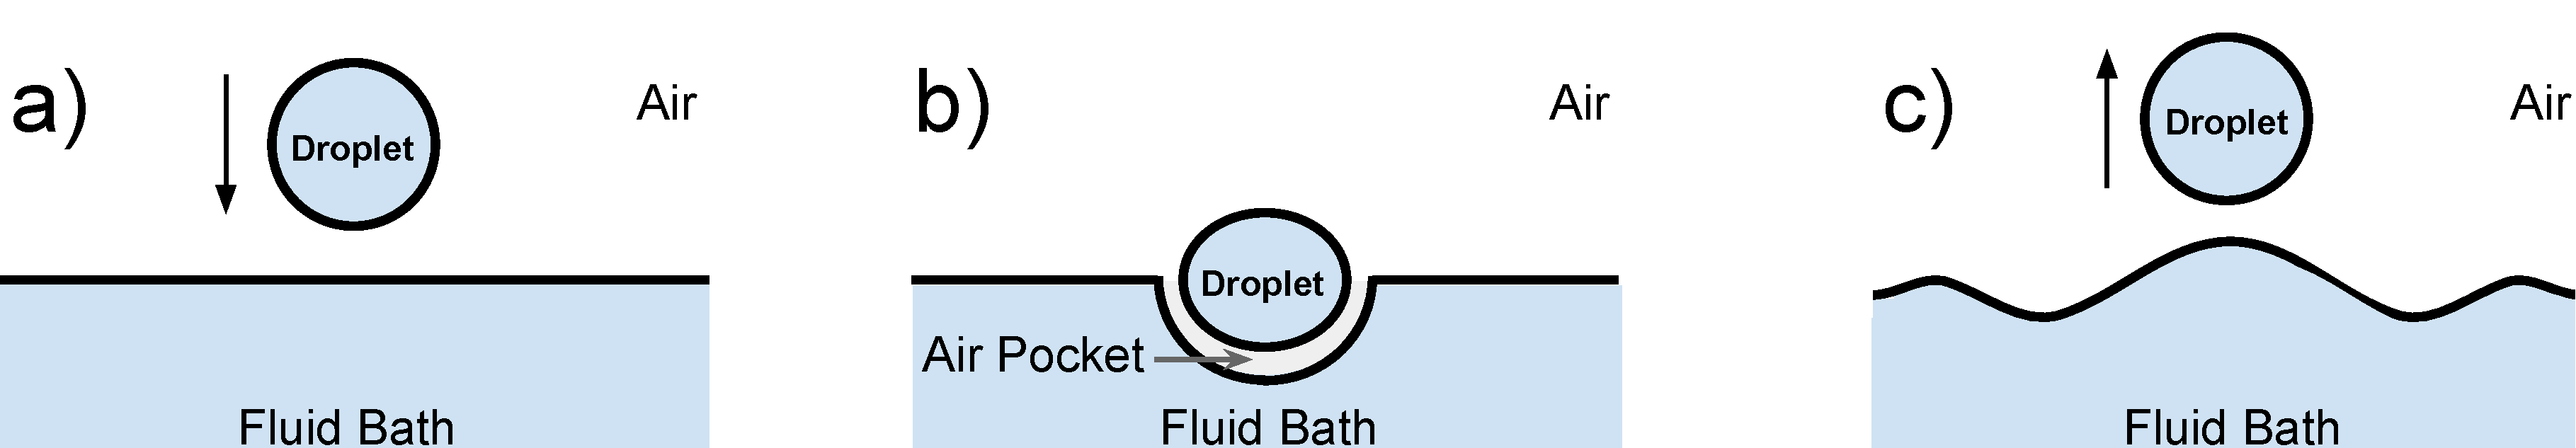
\includegraphics[scale=0.25]{BouncingDroplet.pdf}
	\caption{A depiction of a droplet bouncing on a bath of the same fluid. (a) A droplet falls onto a fluid bath. (b) A film of air gets trapped underneath the droplet. (c) The droplet bounces back up off of the cushion of air leaving behind waves that propagate radially.}
	\label{bounce}
\end{figure}
	    
	    Walker found that a trapped film of air kept the droplet and the bath from touching, as shown in \refFig{bounce}. That is, the droplet is bouncing on a layer of air that's struggling to get out of the way but because the bounce happens so quickly, the fluid droplet and the fluid bath never touch. Walker concluded that the leakage rate of this trapped pocket of air depends on three factors: the surface tension of the fluid in the bath, the viscosity of the droplet and the fluid bath, and the viscosity of the air. The bath must be of uniform surface tension and free from particulate matter floating atop the bath, since both will lead to coalescence. Higher viscosity fluids translate to longer droplet lifetimes, since more viscous fluids keep air from escaping the pocket. Finally, adjusting the frequency and the amplitudes of the vibrations also affects droplet lifetime.\footnote{Reedie Andrew Case ('92) wrote his thesis ``Oil on Troubled Water: The Extension of Floating Drop Lifetimes Due to Interface Vibration" where he looked at droplet lifetime by the frequency of vibration.}   
	     
	    More recent research suggests that a droplet fluid like silicone oil could bounce indefinitely on a vibrating bath\rf{Couder2005a}. The long lifetime occurs not only because silicone oil has a high viscosity, but also because it has a \textit{low} surface tension. A low surface tension is beneficial because it makes the oil bath relatively immune to surfactants (surface acting agents) or contamination which would otherwise make the surface tension nonuniform, and thus create a coalescence event. 

\subsection{Faraday Waves}
	    For a vertically vibrated fluid bath, controlling the amplitude and the frequency of the motion will affect the behavior of the fluid. Depending on a variety of factors (size of bath, fluid in bath, etc.) each system has a specific amplitude (given a specific frequency), which if surpassed, will produce standing surface waves called Faraday waves\rf{Faraday}.\footnote{Faraday waves weren't actually discovered by Michael Faraday; in the footnotes of his paper he cites that they were first observed by Oersted, Wheatstone, Weber, and others. Faraday was just the first high-profile physicist to write about the behavior.}~\footnote{Another Reed thesis, this one titled ``Good Vibrations: A Visual Exploration of Faraday Waves" by Alison Saunders, compares mathematical formulation to experimental results.} A vibrating bath below this critical amplitude, also known as the Faraday instability, will be flat and motionless. A bath with a amplitude greater than the Faraday threshold will have a turbulent surface with ripples and waves. An example of Faraday waves is shown in \refFig{faraday waves}. Adjusting the frequency above the Faraday threshold will change the size and shape of the Faraday waves. Note that Faraday waves can be created either by increasing amplitude to a critical level, or increasing frequency to a critical level.
	    
	    \begin{figure}[h!]
	\centering
	\includegraphics[scale=0.06]{Faraday.JPG}
	\caption{A picture of Faraday waves in a dish of water at $80~\mathrm{Hz}$.}
	\label{faraday waves}
\end{figure}

\subsection{Walking Droplets}
	    
	A bouncing droplet will bounce differently depending on the frequency and amplitude of the vertical vibrations. If the parameters are set just a hair below the Faraday instability, then a very curious motion arises: the droplet seems to ``walk" across the surface of the oil. The droplet is being pushed by its own ripples, a dual effort in which neither can exist without the other. In essence, the walker is both a particle and a wave; a conjunction which has only ever been seen at the quantum scale. 
	  
\begin{figure}[h!]
	\centering
	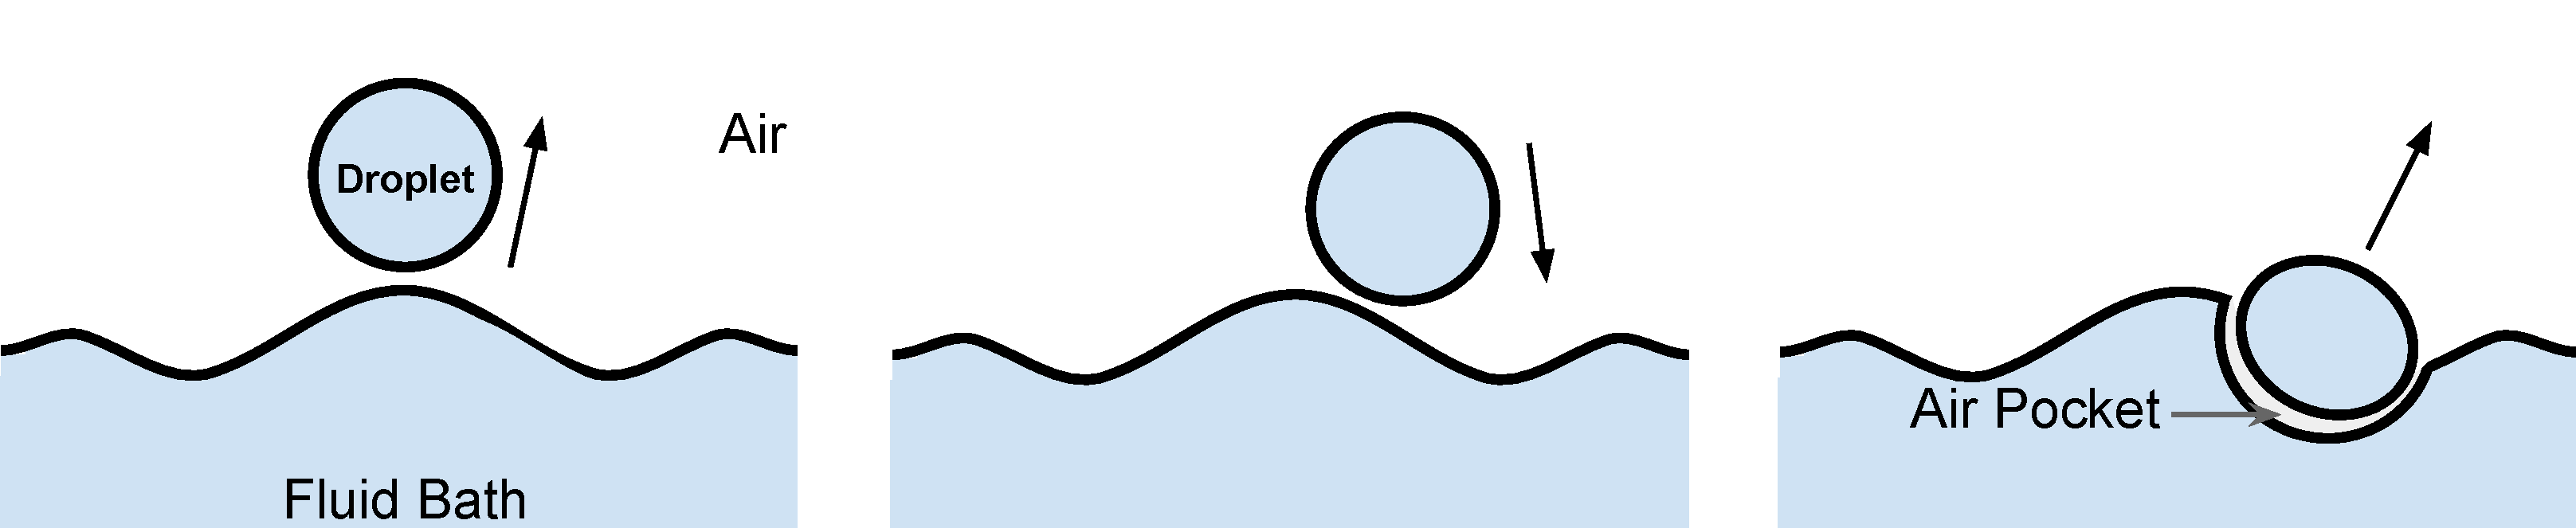
\includegraphics[scale=0.28]{Walking.pdf}
	\caption{A depiction of a droplet walking across a bath of the same fluid.}
	\label{bounce}
\end{figure}
	    
	  
\subsection{Road Map}	  
	  
	Recently, two main groups have been investigating the properties of this unique system. A group at Laboratoire Mati\`{e}re et Syst\`{e}mes Complexes (MSC) in Paris, France, headed by Yves Couder was the first to uncover some of the inherently ``quantum"-like behavior of bouncing droplets, in 2005~\cite{Couder2005b}. Since 2010 John Bush's group at MIT have been adding to the literature by creating a mathematical model, and performing their own investigations of the walker system. Couder, Bush, and others have shown that this system can reproduce double-slit single-particle interference, orbiting, tunneling, quantized orbits, spin, and many more ``quantum"-like effects. 
		
	The thesis documents an experimental investigation into a ``tunneling" behavior of this bouncing droplet system. While only one other study really looks at this aspect~\cite{tunneling}, it falls short of completely examining the tunneling behavior, focusing on barrier width and not examining barrier height. I hope to add to the body of work in this subfield by studying how barrier height affects probability of tunneling.   
	
	This thesis is divided into three main chapters. \textbf{Chapter 1} gives a background of the hydrodynamic quantum analogs along with a brief survey of the relevant literature. In \textbf{Chapter 2}, I lay out the experimental design and explain the setup and the data taking procedures. Finally, the results and conclusions are presented in \textbf{Chapter 3}.	    